%----------------------------------------------------------------------------------------
%	PACKAGES AND OTHER DOCUMENT CONFIGURATIONS
%----------------------------------------------------------------------------------------

\documentclass[fleqn,10pt]{SelfArx} % Document font size and equations flushed left

\usepackage[english]{babel} % Specify a different language here - english by default

%----------------------------------------------------------------------------------------
%	COLUMNS
%----------------------------------------------------------------------------------------

\setlength{\columnsep}{0.55cm} % Distance between the two columns of text
\setlength{\fboxrule}{0.75pt} % Width of the border around the abstract

%----------------------------------------------------------------------------------------
%	COLORS
%----------------------------------------------------------------------------------------

\definecolor{color1}{RGB}{0,20,20} % Color of the article title and sections
\definecolor{color2}{RGB}{0,20,20} % Color of the boxes behind the abstract and headings
\definecolor{deep_blue}{HTML}{006092}
\definecolor{normal_blue}{HTML}{1368c7}
\definecolor{light_blue}{HTML}{339fd6}
%----------------------------------------------------------------------------------------
%	HYPERLINKS
%----------------------------------------------------------------------------------------

\usepackage{hyperref} % Required for hyperlinks
\hypersetup{hidelinks,colorlinks,breaklinks=true,urlcolor=color2,citecolor=color1,linkcolor=color1,bookmarksopen=false,pdftitle={Title},pdfauthor={Author}}



% The following packages can be found on http:\\www.ctan.org
\usepackage{graphics} % for pdf, bitmapped graphics files
\usepackage{epsfig} % for postscript graphics files
\usepackage{mathptmx} % assumes new font selection scheme installed
\usepackage{times} % assumes new font selection scheme installed
\usepackage{amsmath} % assumes amsmath package installed
\usepackage{amssymb}  % assumes amsmath package installed
\usepackage{pgfplots}
\usepackage{longtable}
\pgfplotsset{width=8cm, compat=1.9}


\begin{document}
%%%%%%%%%%%%%%%%%%%%%%%%%%%%%%%%%%%%%%%%%%%%%%%%%%%%%%%%%%%%%%%%%%%%%%%%%%%%%%%%


\begin{titlepage}
   \begin{center}
       \vspace*{0.5cm}

       \color{black}{\huge 2019 AUVSI SUAS Competition }\\
       \vspace{0.2cm}
       \color{light_blue}\textbf{ \Huge Condor Technical Design Paper} \\
 
      \vspace{0.5cm}
      
        \begin{figure}[h]
        \includegraphics[width=\linewidth]{figures/CondorMaiden.jpg}
        % \caption{Condor}
        % \label{fig:Condor}
        \end{figure}
        
        % \hline
        \vspace{0.5cm}
       \color{normal_blue}\textbf{Unmanned Aircraft System Design Team} \\
        % \vfill
        \color{black}
        University of British Columbia\\
        2329 West Mall \\
        Vancouver, BC Canada V6T 1Z4 \\
        \texttt{info@ubcuas.com}


        \vspace{0.5cm}

        %%%%%%%%%%%%%%%%%%%%%%%%%%%%%%%%%%%%%%%%%%%%%%%%%%%%%%%%%%%%%%%%%%%%%%%%%%%%%%%%
% \twocolumn
\begin{flushleft}
{The University of British Columbia Unmanned Aircraft Systems engineering student team (UBC UAS) is a multidisciplinary group of students spanning multiple faculties, including Engineering, Forestry, Science and Business. It strives to be at the cutting edge of unmanned aviation technologies, working with industry and government to use unmanned aerial systems in a broad spectrum of disciplines and applications.}
\end{flushleft}

\endinput

%%%%%%%%%%%%%%%%%%%%%%%%%%%%%%%%%%%%%%%%%%%%%%%%%%%%%%%%%%%%%%%%%%%%%%%%%%%%%%%%
        
        \vfill
   \end{center}
\end{titlepage}
\twocolumn
\endinput
% \twocolumn
\onecolumn
\newpage
\tableofcontents
\listoffigures
\newpage
\twocolumn

%%%%%%%%%%%%%%%%%%%%%%%%%%%%%%%%%%%%%%%%%%%%%%%%%%%%%%%%%%%%%%%%%%%%%%%%%%%%%%%%
\twocolumn
\section{System Engineering Approach}
\label{sec1:introduction}

%citation example: \cite{c1}
\subsection{Mission Requirement Analysis}
UBC Unmanned Aircraft Systems (UAS) went through thorough research and development, design, manufacturing and testing phases to ensure a full robust system. Using the Mission Success Analysis table below, the team determined which tasks were both reachable and yielded the greatest return with justification. All tasks listed as “High” will be attempted, while “Medium” may be attempted and “Low” will not be attempted. See table 1.


\subsection{Design Rationale}
    \subsubsection{Environmental Factors}

     This year the team approached projects with a mindset of fulfilling minimum requirements for competition before building on them to expand capabilities or reliability. Long shot ideas were minimized in favor of a faster iterative design process. This resulted in working systems much earlier in the year that allowed all system level problems to arise early enough that they could be dealt with.

    Given UBC UAS’ location in the heart on Vancouver, fixed wing flight locations are limited. Several locations within 15 minutes of the team’s design space offer space for multi-rotor testing, while fixed wing testing grounds are at least 45 minutes away and require further coordination with external groups. 
    
    \subsubsection{Aircraft Choice}
    The 2019 AUVSI SUAS competition presents a very unique engineering challenge in terms of distance, time, and accuracy requirements of the chosen aircraft design. Given the mission requirements for 6+ miles of flight and high accuracy payload drop it was determined that the most capable system for mission success would likely be some sort of VTOL. UBC UAS instead opted for a multirotor on the basis of significantly improved payload drop accuracy, easier testing, and simpler obstacle avoidance routing. Previous experience with VTOL development proved that it was not ideal to focus all efforts on such a long shot and instead to focus on reliability as stated above. This presented a number of other challenges in order to meet mission distance and time requirements. 


    \begin{figure*}\centering
    \includegraphics[width=0.9\textwidth]{table/table_1.png}
    \caption*{}
    \label{fig:msa}
    \end{figure*}



\endinput
%%%%%%%%%%%%%%%%%%%%%%%%%%%%%%%%%%%%%%%%%%%%%%%%%%%%%%%%%%%%%%%%%%%%%%%%%%%%%%%%
%%%%%%%%%%%%%%%%%%%%%%%%%%%%%%%%%%%%%%%%%%%%%%%%%%%%%%%%%%%%%%%%%%%%%%%%%%%%%%%%

\section{System Design}
\label{sec2:design_analysis}


\subsection{Aircraft}
\begin{subsubsection}{Power System}
As stated previously, the 2019 mission requirements for distance and time constraints created significant challenges in finding a capable power system. Several weeks of initial design simulation was performed with the online tool ecalc.ch. This allowed the team to quickly simulate a wide number of possible configurations combining motors, electronic speed controls (ESC's), and propellers. Several configurations were found that meet the distance requirement but it wasn’t until the team looked at fixed wing propellers (mounted on higher speed motors) that a viable configuration was found. The high pitch of fixed wing propellers, slightly higher Kv motors, and a higher voltage power system, allowed the multirotor to sustain thrust at high speed. Once this characteristic was identified the available propellers were quickly limited to the 20x13" from APC Propellers as no other comparable propeller was found. This paired with a motor in the 150-200kv range operating at 50v (12s LiPo) provided the necessary thrust. A final configuration using 22Ah of battery and a choice of two motors and ESCs satisfied all of the mission’s requirements in simulation. 

The APC 20x13” props were placed on a dynamometer for validation of specifications and curve fitting RPM to thrust values. UBC UAS tests showed the propeller performing at or above the data supplied by APC and thus met the team’s needs for the mission. Mapping RPM to thrust allowed testing at higher thrust levels as the team’s dynamometer was limited to 5kg, while measuring of higher RPM values was simply measuring the ESC output frequency with a conversion factor. 

\vspace{5mm}
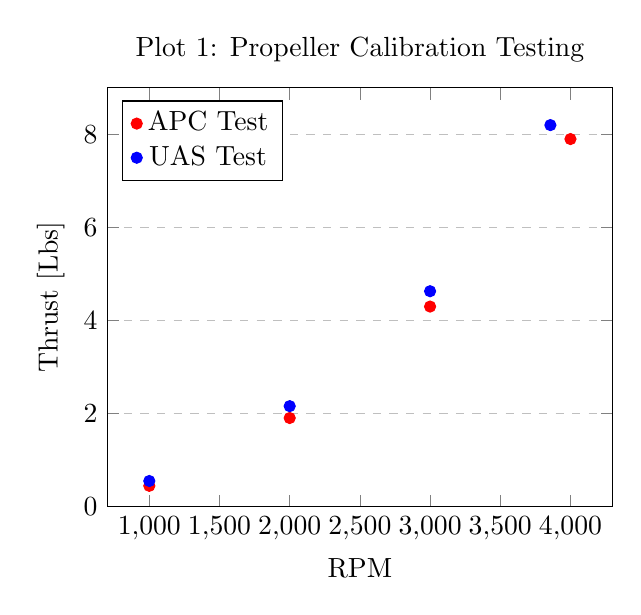
\begin{tikzpicture}
\label{Fig:propeller_calibration_testing}
\begin{axis}[
    title={Plot 1: Propeller Calibration Testing},
    xlabel={RPM},
    ylabel={Thrust [Lbs]},
    %xmin=0, xmax=100,
    ymin=0, ymax=9,
    %xtick={0,20,40,60,80,100},
    %ytick={0,20,40,60,80,100,120},
    legend pos=north west,
    ymajorgrids=true,
    grid style=dashed,
]
\addplot[only marks, color=red]
    coordinates {
    (1000,0.447)(2000,1.905)(3000,4.3)(4000,7.9)};
\addplot[only marks, color=blue]
    coordinates {
    (1000,0.551)(2000,2.16)(3000,4.63)(3857,8.2)};
\legend{APC Test,UAS Test}
\end{axis}
\end{tikzpicture}

\paragraph{Testing}
Final motor and ESC decisions required bench testing of components. One of each T-motor (MN601s-170kv and MN605s-170kv) motor was tested along with both the traditional T-motor Flame 60A HV and the newer Alpha 60A HV FOC (Field Oriented Control) ESCs. Both ESCs were tested for response time and efficiency in terms of thrust per watt of input power (See Plot 2: ESC Efficiency Testing). While there was not a significant difference in either of these metrics the Alpha ESCs were chosen because of their data logging capabilities and over power limiter. This over power limit is important as bench calculations showed the possibility of drastically overpowering the motors at the very top of the throttle curve. 

    % \begin{figure*}\centering
    % \includegraphics[width=0.9\textwidth]{table/table_1.png}
    % \caption*{}
    % \label{fig:msa}
    % \end{figure*}


\vspace{5mm}
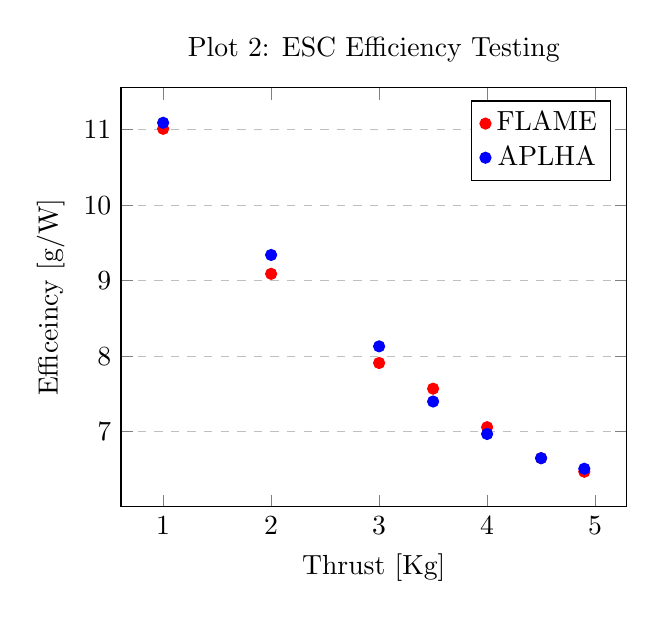
\begin{tikzpicture}
\begin{axis}[
    title={Plot 2: ESC Efficiency Testing},
    xlabel={Thrust [Kg]},
    ylabel={Efficeincy [g/W]},
    %xmin=0, xmax=5,
    %ymin=0, ymax=9,
    legend pos=north east,
    ymajorgrids=true,
    grid style=dashed,
]
\addplot[only marks, color=red]
    coordinates {
    (1,11.01)(2,9.09)(3,7.91)(3.5,7.57)(4,7.06)(4.5,6.65)(4.9,6.47)};
\addplot[only marks, color=blue]
    coordinates {
    (1,11.09)(2,9.34)(3,8.13)(3.5,7.40)(4,6.97)(4.5,6.65)(4.9,6.51)};
\legend{FLAME,APLHA}
\end{axis}

\end{tikzpicture}

Both motors from T-Motor were also tested for total available thrust and power consumption at cruise thrust. Cruise thrust was calculated as a function weight and speed with simplified drag equations. It was found that the increased weight and power consumption of the MN605s projected to reduce the flight time by less than a minute. The additional power of the MN605s was deemed to be desirable as it improved controllability, and there was some uncertainty in exact final all up weight for the aircraft.  

\subsubsection{Frame}
In order to accommodate such a heavy aircraft and power system, a strong and more importantly, stiff frame was required. From previous experience, the team found that a frame that is not sufficiently able to deal with vibrations can prove to be near impossible to tune for stable flight. This led the team to opt for significantly larger frame tubes than have been used in the past at 30mm diameter. Additionally the arms were shortened as much as possible. The center plates, forming a standard “sandwich” design, were constructed out of $1/4$” aluminum - water jetted to remove all extraneous material and weight.  The center plate was also made as small as possible in overall dimensions to reduce bending moments. The simple and classic sandwich design uses very few unique parts making it very quick to assemble as easy to keep spare parts on hand.  

A strong separation was made between payload systems and flight systems on the aircraft, for the purpose of modularity. This meant a completely separate removable center plate for payload systems that sits under the aircraft and is secured with 4 bolts and a single multi-pin cable. This configuration offers significant benefits in parallel development efforts, as well as the ability to quickly switch out payloads as will be necessary for UBC UAS’ second Canadian competition in May that requires a completely different payload. 

Refer to Figure 1 for airframe dimensions.

\begin{center}
\begin{tabular}{c c c } 
 \hline
 Property & Metric & Imperial \\ 
 \hline
 Overall Width & 1508mm & 59in \\ 
 Overall Width (w/o Props) & 1000mm & 39in \\ 
 Maximum Takeoff Weight & 11.5 kg & 25 lbs \\
 Cruise Speed & 12 m/s  & 21 knots \\
 Maximum Speed & 25 m/s & 49 knots \\
 Operational Range & 11.3 km & 7 Miles \\
 Max Flight Time & \multicolumn{2}{c}{30 min} \\
 Batteries & \multicolumn{2}{c}{16-24 Ah, 12S batteries} \\
 Total Power capacity & \multicolumn{2}{c}{1020Wh} \\
\end{tabular}
\end{center}

\begin{figure}[ht]\centering
\includegraphics[width=\linewidth]{figures/Frame}
\caption{Frame}
\label{fig:frame}
\end{figure}


\end{subsubsection}

\endinput

%%%%%%%%%%%%%%%%%%%%%%%%%%%%%%%%%%%%%%%%%%%%%%%%%%%%%%%%%%%%%%%%%%%%%%%%%%%%%%%%
\subsection{Autopilot}
\subsubsection{Flight Control System}
%Check Google docs bullet points

In this year's competition vehicle the team opted to use the Pixhawk 2. This flight controller will be replacing the Pixhawk 2.4.8 by 3DR. This flight controller was chosen not only for its triple redundant IMU system, but also since it has more ports, better connectors and an internal IMU damping system. The Pixhawk 2 has interface supports for all the sensors and actuators that are used in the system, as well as the telemetry radio. 

The team is using Ardupilot as its flight controller software. It was chosen due to its community support on forums and its code base reliability. Even though Ardupilot is a open source program, the development team conducted flight testing on each of their new releases. Ardupilot provides precise waypoint navigation, autonomous takeoff, and autonomous landing: the waypoint navigation feature will help object avoidance, task rescheduling and altering the mission route. The team can also avoid pilot takeover penalties from autonomous landing/takeoff.

\endinput
\subsubsection{Object Avoidance and Path Planning}
The algorithm for obstacle avoidance needs to avoid cylindrical objects in a 3D space. Specifically, it needs to be able to avoid obstacles by going around them - this is more efficient when doing the automatic flight portion. However, for the ODLC survey, the aircraft should fly over the obstacles to keep the survey path intact. The algorithm needs to take into account the size of the aircraft plus an additional safety factor during the avoidance in case of GPS accuracy when considering possible collisions and acceptable routes .

All the algorithms are housed in the ‘avoidance’ module within the GCOMv2 software in the GCS. It contains a variety of REST endpoints to perform routing on the map frontend. Some preprocessing is done as soon as the information is gathered from interop, however the actual routing is done on demand to keep system resource use efficient. Once routing is complete, the waypoints are cached to the database so that future calls don’t need to perform the routing again. There is an endpoint to force a re-compute of the route, as well as too write a custom path to the database cache. This allows for user modifications if the computer generated route is unsatisfactory.

The core algorithm for the avoidance and routing is based of a modified version of the A* algorithm called L1. The A* algorithm treats the flight space as a 2D grid, and is computed as a graph. The A* algorithm starts at the start node of the graph then recursively tries all possible routes through the edges of the grid, however it prioritizes trying the path that is both the shortest path so far and what it thinks is the best possible next path. This best next path is controlled by a heuristic. In this case it is the straight line distance from the node to the goal. The advantage of using this path finding algorithm to do obstacle avoidance is that any combination or layout of obstacles can be handled without the inclusion of special rules or edge cases. It also works easily in three dimensions, so it can handle the full flight space and all of the problem requirements.

\begin{figure}[h]\centering
\includegraphics[width=\linewidth]{figures/OA_1.png}
\caption{The target route. Flyzone in red, obstacles in yellow.}
\label{fig:OA_1}
\end{figure}

However, for UAS's use case the base A* algorithm was improved. Inspiration was taken from the L1 improvement of the A* algorithm. Mainly, the steps of pre-processing the grid and reducing the number of potential paths that need to be considered. In the case of this problem, the points of the 1m by 1m grid were reduced to just the nodes of: the waypoints given, a few points close to the obstacles and points around the inside edge of the flyzone (Figure 2). This greatly reduces the number of points and paths considered and considerably speeds up the routing. To further speed up the routing, the edges of the graphs between the points were pre-computed to reduce the pathfinding time even more. This is done asynchronously immediately after the mission information is gathered from the interop server.

\begin{figure}[h]\centering
\includegraphics[width=\linewidth]{figures/OA_2.png}
\caption{The reduced graph of nodes used in the A* search.}
\label{fig:OA_2}
\end{figure}

In Figure \ref{fig:OA_2}, note the clusters of overlapping nodes around the obstacles. To enable 3D searching, but still reduce the number of nodes tested, the search nodes are placed just outside the mid height of the obstacle, and just above the top of the obstacle. On the map they appear as overlapping nodes.

When testing the algorithm, several key edge cases between two points were considered:
\begin{itemize}
\item Free Path between two points.
\item Single obstacle.
\item Multiple obstacles in a line.
\item Multiple obstacles coincident.
\item Multiple obstacles overlapping.
\item Multiple obstacles randomly dispersed.
\item Going around and going over obstacles.
\item Flyzone jutting out between the two points.
\item Combinations of the above.
\end{itemize}

\endinput




%%%%%%%%%%%%%%%%%%%%%%%%%%%%%%%%%%%%%%%%%%%%%%%%%%%%%%%%%%%%%%%%%%%%%%%%%%%%%%%%
\subsection{Communication}
\subsubsection{Antenna Tracker}

\begin{figure*}[ht]\centering
\includegraphics[width=\linewidth]{figures/Systems_Link_Diagram.png}
\caption{Systems Link Diagram}
\label{fig:systems_link_diagram}
\end{figure*}


The antenna tracking system orients the antennas towards the UAV. This ensures a constant clean and strong link is established between the ground and the UAV. Its main purpose is to facilitate real-time image transfer and first person video (FPV).

The tracker receives GPS coordinates and the altitude of the UAV, encoded via the Mavlink protocol, over the RFD900+ telemetry radios. DroneKit-Python SDK (Software Development Kit) is used to read the RFD900+ data over a serial connection to a raspberry pi. A vector is then derived based on the position and altitude of the tracker, providing a target antenna orientation. The tracker has two degrees of freedom which are rotation in both yaw and pitch. To generate motion in these directions, two Dynamixel smart servo motors are used. 

The tracking station is placed on a 2m high tripod. Batteries, motor controllers, and the Raspberry Pi are all mounted on top of the tripod to reduce wiring complexity. A vertical rod coaxial to the tripod houses wires and is the axis for yaw rotation. Gears are used instead of belt drive in order to reduce slipping and allow for lighter and more flexible materials. The gear ratio of 3:7 from motor was selected for the yaw direction to allow for fast and accurate tracking of the drone, while maintaining stability of the station. The second motor in the pitch direction is geared 1:1 to a horizontal shaft, which orients the FPV receiver and yagi antenna towards the drone. 

The antenna tracker methodology of using the received signal strength indicator (RSSI) was also explored during the research stage of the project. The idea was to use the RSSI of the RFD telemetry radios as an indicator for finding the vector between the UAV and tracker. This method proved to be more complicated as the RSSI signal was highly noisy. Furthermore, the model proved to be outside the proposed budget, hence the GPS coordinates methodology took precedence. 


\subsubsection{Ground Control Station}
An in-house Ground Control Station(GCS) was developed, shown in figure \ref{fig:map_gui}. The GCS provided user-friendly interface for operators to connect to the interoperability server, displaying obstacles and waypoints in real time. 

In addition to our main Ground Control Station, the team also uses Mission Planner to control the autopilot, update the flight plan and configure the autopilot. Mission Planner supports functions like retrieving the telemetry data and controlling the camera gimbal which simplify some of the controls. Since the GCS is still under development, it cannot fully replace Mission Planner, so in the competition both Mission planner and the GCS will be used in tandem. 

The ground control station maintains constant communication with the UAV. It is connected directly to the antenna tracker over Ethernet network, receiving data from the Ubiquiti M2 Bullets. The Bullets create a point-to-point network (2.4GHz) between the tracker and quadcopter. GCS receives images for image processing and also receives telemetry data over the RFD900+ radios to process and send to interop server.  

\begin{figure}[ht]\centering
\includegraphics[width=\linewidth]{figures/map_gui.png}
\caption{Ground Control Station Interface}
\label{fig:map_gui}
\end{figure}

\subsubsection{UAV Pilot and Rover Supervisor}

The UAV pilot will have manual control of the UAV via the Dragonlink transmitter/receiver, operating on 433MHz. The Rover supervisor will have failsafe control over the Rover via the Taranis transmitter/receiver operating on 2.4GHz frequency. Refer to the Figure 4 for a full communications overview. 
\endinput

\subsection{Cyber Security}
\begin{figure*}[ht]\centering
\includegraphics[width=0.8\textwidth]{table/Table_2_cyber_security_attacks.PNG}
\caption*{}
\label{fig:cs}
\end{figure*}
The UAS system is vulnerable to three types of attacks: hardware attacks, wireless attacks and sensor spoofing. 

Hardware attacks includes attacks where man-in-the-middle (MitM) directly attacks the components of the UAV, such as physically hijacking the UAV. Wireless attacks are when the attacker intercepts, modifies, fabricates identity or denies of service (DoS) the communicate links or nodes. Sensor spoofing is when attackers interrupt the UAV’s on-board sensor data.



The team enhanced the security of its system by adding multiple layers of protection to prevent threats from different aspects. Table 2 illustrates four major security threats with their severity level identified (1 being the highest) within the current system design and solutions the team has implemented. The main focus has been to address Wireless attacks. See table 2.



% \onecolumn
% \begin{table}[t]
%     \centering
%     \normalsize
%     \label{tab:cyber_security}

%     \begin{tabular}{p{1cm} p{4cm} p{3cm} p{5cm} p{5cm}}
%     \hline
%     Severity Level & Attack & Types of attack & Threat description & Solution \\ 
%     \hline
%     1&RFD900 Radio Modem for telemetry and commands&Wireless attack&
%     Interference from nearby signals on similar frequencies with the possibility of unauthorized control to the drone, and from MitM with one of the wireless attack types. 
%     & \begin{enumerate}
%         \item AES encryption on the traffic \item Use of the Mavlink 2 protocol which includes a signed encryption bit
%     \end{enumerate} \\ 
    
%     \hline
%     2&Ubiquiti Bullet for ground to drone communications&Wireless attack&MitM with one of the wireless attack types. & SSH with with public-private key encryption \\
%     \hline
%     3&Ground control server router/network&Wireless attack& MitM with one of the wireless attack types. &WPA2 encryption \\
%     \hline
%     4&GPS spoofing& Sensor spoofing&GPS data was received from MitM instead of reliable source. & Use of RTK system, and Failsafe for losing control\\
%     \hline
%     5&
%     Physical hijacking &Hardware attacks&UAV is hijacked physically by MitM&Trigger failsafe to avoid further damage.  \\
     
%     \end{tabular}
% \end{table}
% \twocolumn

\endinput
%%%%%%%%%%%%%%%%%%%%%%%%%%%%%%%%%%%%%%%%%%%%%%%%%%%%%%%%%%%%%%%%%%%%%%%%%%%%%%%%

\subsection{Airdrop System}
\paragraph{Overview} The aim of the Airdrop system is to deliver a Unmanned Ground Vehicle (UGV, same as Rover) to a designated location and also provide real time images to the ground using on-board computer and communication modules. For the delivery, after the waypoint capture mission, which may goes up to 4 miles in distance, Condor will arrive at the drop location that is previously given to us. Then the payload system will lower the Rover while the aircraft stays loitering, and use a pulley system to release the Rover autonomously before retrieving the rope. Then the system will idle until the end of the mission. For the image transfer task, after the aircraft enters the search area, the camera will start taking images at a preset interval while the aircraft is at this specific flight area. The image is tagged on-board with the real-time data from flight controller and then transferred to the GCOMv2 server computer immediately.  
% read
\paragraph{System Component}
Payload system consist of 3 parts: 
\begin{itemize}
    \item Imaging system, UGV and air delivery system.  The imaging system has a camera, 1 axis gimbal, raspberry pi, bullet, POE ejector and image transferring software. 
    \item Rover consists of UGV, UGV control software and water bottle. 
    \item Air delivery system has a Winch, winch control electrical system, winch control software and various hardware to mount UGV. 
\end{itemize}
%read


\subsubsection{Winch subsystem}
\paragraph{Requirements}
The requirements of the winch subsystem were based on the aircraft's capability and competition's operation and flight time window. 
\begin{itemize}
    \item Weight cannot exceed 1 kg.
    \item Power consumption: limited to 5V and 12V, parallel to the aircraft's PCB.
    \item Operate at the minimum competition flight attitude, which is 30m MSL.
    \item Can withstand 5G acceleration, up to 25m/s.
    \item Complete the whole airdropping operation under 1 minute.
\end{itemize} 

The team considered three designs for deploying the UGV from Condor: parachute drop, pulley system or a direct drop. A direct drop was eliminated from the list as Condor has a minimum altitude - one that is too high to safely drop the. Since the parachute is the lightest option when considering weight, the team tested it by prototyping different types and designing one that yields the highest precision on its drop location. It needs to be ensured the rover is dropped at sufficiently low velocity. The velocity attained via the parachute was too high to merit a safe drop. Additionally, a parachute would require the UGV to be encompassed with some protective material to survive the drop, which would ultimately cause the 1kg UGV weight limit to be exceeded. Testing revealed the parachute to be too unpredictable and difficult to control. Thus, a pulley system was designed. The pulley can control the releasing speed of the 1kg UGV from the lowest flight altitude.
%read

\paragraph{Design Consideration}
The winch system has two tasks: release the Rover and retract a rope. The first task uses a servo controlled brake and motor drag system, and the second task uses the same motor to recover the rope. Both systems are dependent on an encoder to measure the length of the rope used. %read

The winch system is designed based around limiting the rotating drum’s maximum RPM (Revolutions Per Minute) to obtain precise measurement of length and instant velocity and to minimize the weight. To find the size of the drum, it was first assumed that releasing and retracting will take 15 seconds and 5 second each from a 30 meter drop height. During prototyping, our first iterations encoder worked the best at around 400 RPM, however later on a better encoder that raised the RPM cap to over 1000 was acquired. When determine the retracting RPM, it was found that when over 600 RPM, the rope will start over-retracting and cause rope interleaving; slower RPM leads to longer retracting time and motor under-powering. Drum size was based on estimating the diameter x with: $$600 RPM \cdot \frac{15s}{60s} \cdot (x cm \cdot \pi) = 3000 cm$$ which results in about 6.3 cm in diameter. 
%read

Next a gear train was designed to make sure that the RPM for the encoder was within its optimal measurement range. For this stage Cylewet’s CLT1062 encoder was used, which provides 20 pulses or 40 ticks per revolution. This relatively cheap and light encoder was elected based on estimations of system limitations. Considering the worst case of free falling for 20 meters, which result in about 20m/s of velocity:
$$20 m/s \rightarrow 2,000 cm/s \rightarrow 2 cm / ms \approx  0.1 resol/ms \rightarrow 4 ticks/ms$$
Given the maximum reading frequency of the Teensy Encoder module of 50kHz, which is less than 1 ticks/ms, it was decided that the encoder did not need to be geared down.

As for choosing the motor, a DC motor was chosen over a stepper motor due it’s light weight and faster no load RPM. Although a stepper motor gives full control over the releasing with it’s high stall torque($\approx$ 1.5kg * 6.3 cm ~ 9.45 kg cm), with the voltage and current limitation, the stepper motors that meets this requirement are at least 500 grams. In addition it's low RPMs are not able to meet the operation time window. Therefore the following motors were tested: (RPM/stall torque) 300 RPM/15kg$\cdot$cm, 1k RPM/6kg$\cdot$cm, 3.5k/3kg$\cdot$cm and 10k RPM/3kg$\cdot$cm. It was found that the 1k RPM with 6 kg$\cdot$cm stall torque motor can meet the retracting speed requirement and at the same time provides noticeable slow down when releasing. The drum motor was geared up by 1.4 to give more control over the retracting. To compensate for motor’s low stall torque, a servo trigger friction brake was added that is capable of stopping the drum with only 30 cm delay after a 2 second free fall.
Refer to Table 3 for specific measurements. 

\begin{figure}[h]\centering
\includegraphics[width=\linewidth]{table/Table_3_Air_delivery_system_design.PNG}
\caption*{}
\label{fig:airdrop_design}
\end{figure}



\paragraph{Operation}
The winch subsystem has two modes: manual mode allows the pilot to trigger the winch mechanism using a channel switch on the flight controller where as autonomous mode gets triggered automatically when the quadcopter reaches the desired GPS location. On the flight side, the on-board computer (Raspberry Pi 3) triggers the winch operation. The Teensy 3.5 microcontroller begins the releasing operation - it sets a servo based braking mechanism to its release position, and the motor is powered at the same time to generate a counter torque. A rope is released, whose length is measured with a rotational encoder. The encoder measures the rotational resolutions of the drum and calculates the approximated distance and instant velocity of the releasing. If the dropping speed exceeds a certain threshold, the braking system and motor will adjust the error with a PD controller. Once the winch system has detected that the Rover has reached the ground or the releasing altitude has met the length of the rope released, a linear actuator will release the geared slider on the Rover and detach the rope. The rope is then retracted back to the aircraft, finishing up the airdrop operation in a physically and electrically stable state. 
%read

\begin{figure}[h]\centering
\includegraphics[width=\linewidth]{figures/PayLoad.png}
\caption{Winch subsystem Diagram}
\label{fig:winch_diagram}
\end{figure}

\paragraph{Testing}
To test the winch system, first an isolated testing environment was set up to make sure that each components work as expected, then they were integrated with a testing aircraft and finally Condor. After each component was tested, an integrated test to select the releasing algorithm and controllers was conducted by releasing a similar payload from a high altitude location (A 3rd floor sundeck), and the performance of the dropping was recorded. In the end, it was found that the system can be controlled only with a proportional differential(PD) controller.  

For aircraft testing, the testing multirotor was set to loiter at 30 meters and the winch underwent several tests with various dropping speed, different controller algorithms and dropping altitudes ranging from 20 to 40 meters. The ground personnel observed and recorded the dropping accuracy, the stability of the drop and the integrity of the payload. In the end it was concluded that 15 seconds dropping window not only feasible, but also was the configuration with one of the most stable performances, as the aircraft wasn't as influenced from the rapid controller error correction and the drop was efficient due to it's relatively short drop time. Although the oscillation created at the end of the 30 meter long rope only seems to be a major problem in windy weather, some manual tuning on the PD controller will be conducted on site depending on the wind conditions, since the winch can reliable perform a high speed drop and completely stop the release within about half a meter from a 2 second free drop. 
%read

\subsubsection{Unmanned Ground Vehicle}
\paragraph{Requirements} 
We set design requirements for the rover to meet or exceed the competition requirements. 
\begin{itemize}
\item The weight is not to exceed 1 kg, with the water bottle attached. 
\item The rover should autonomously drive to a specified location.
\item In case of loss of communication or driving out of specified boundaries, the rover is to stop driving within 30 seconds. 
\item The speed of the rover is limited to 10 miles per hour.
\end{itemize}

To meet these requirements of autonomy and emergency shutoff, it was additionally required that the rover contain a GPS receiver, radio receiver, and motor controller. 

\paragraph{Design Process and Mechanism Description} 
Besides the performance goal of delivering a water bottle, a great deal of freedom was awarded in designing the rover. Prototypes with three wheels and four wheels, and a variety of attachment systems to secure the rover to the UAV in flight were considered. Ultimately, the decision to use four wheels was made. This allowed the team to design a smaller base-plate and a shorter rover, since the water bottle can be positioned between the wheels (See Figure 6). Furthermore, having four wheels improves stability, which is greatly beneficial on uneven terrain. A rack-and-pinion design at the top of the rover was used for the detachment mechanism, which was chosen for its reliability in actuation. The rack was modified to allow for the rover to attach at three non-collinear points, which increases resistance to vibrations and changes in direction during flight. 

3D printing was harnessed extensively to perform rapid prototyping and to achieve tight fits around other electronic components, which would not have been feasible with traditional manufacturing methods. As a result, as shown in the diagram below, the rover’s components are packed tightly into a space-efficient design (Figure 7).

\begin{figure}[H]\centering
\includegraphics[width=\linewidth]{figures/Rover_Diagram.png}
\caption{Rover subsystem Diagram}
\label{fig:systems_link_diagram}
\end{figure}

\paragraph{Testing Methods} 
The performance of the rover system itself was tested by letting it drive autonomously to specified GPS coordinates in a field. To test the rover as a component of the entire payload system, the detachment mechanism was first tested by flying the UAV at a low height and lowering the rover, and eventually flying the UAV in normal operating speeds and accelerations and testing that the rover could withstand the vibrations and changes in direction typical to UAV flight.

\endinput


%%%%%%%%%%%%%%%%%%%%%%%%%%%%%%%%%%%%%%%%%%%%%%%%%%%%%%%%%%%%%%%%%%%%%%%%%%%%%%%%
\subsection{Vision System System}
\subsubsection{Imaging System}
\paragraph{Requirements}
Imaging system: 
\begin{itemize}
    \item Limited to using raspberry Pi 3 B+ as on-board computer due to budget.
    \item The delay of image transfer should be less than 1 second, ignore wireless transfer time. 
    \item Images should be tagged in real time with no delay. 
\end{itemize}
\paragraph{Camera}
%Identify the camera used by UAS and describe its capabilities, provide a detailed analysis to demonstrate that the chosen camera can resolve objects of the size required by the competition.%

The team's budget for camera was approximately \$800 CAD, and most of the high-end research cameras cost more than \$1000 CAD without the lens. The goal is to capture high resolution images to yield a wide ground area coverage per image, all the while staying under the proposed budget. Digital single-lens reflex (DSLR) cameras with their large Complementary metal–oxide–semiconductor (CMOS) sensor fit the team requirements. Refer to Table 4 for all the cameras under consideration.

\begin{figure}[H]\centering
\includegraphics[width=\linewidth]{table/Table_4_camera_specs.PNG}
\caption*{}
\label{fig:cs}
\end{figure}

After taking the size of the camera into consideration, the SONY A5100 is clearly the best choice since although A6000, A6300 and A5100 all have similar image quality, but unlike the rest the the Sony A5100 doesn't use a optical view finder, which greatly reduced it's size,  weight and price. Although it's battery life is not ideal for the long flight time, an external charging port is used to replace the internal battery to overcome that limitation. What's more, Sony A5100 is one of the cameras supported by gphoto2 API, which simplified it's programming interface. 

\paragraph{Gimbal} 
Five different gimbal configurations were considered: using brushless motors or servo motors, with 2 axis, 1 axis or no gimbal at all. The major requirements were the weight and angle of operation. As per flight data, Condor has a maximum forward bank of 35$^{\circ}$, up to 40$^{\circ}$ when flying at 25m/s. Consequently, the 40$^{\circ}$ pitch angle in forward and 15$^{\circ}$ in backward were reserved; images will not be captured when flying backwards. Next, the gimbal control was chosen from three options: use a dedicated controller like BASECAM BGC, create a custom controller from scratch or use Mission planner's gimbal control feature. Optimizing the weight of payload, the team decided to go with the custom option, using a small and light weight servo motor. The chosen camera, Sony A5100, has a length x height of 110 x 63mm. To allow the gimbal to enclose this large camera and still function properly, the decision to use a single axis gimbal was made. This axis is being used to stabilize the large angle forward pitch. Any small roll angles will be accounted for through the software calibrating the images. 

\paragraph{Image transfer software}
During flight, images are taken by the UAV and geotagged with relevant flight data — latitude, longitude, altitude, heading, roll—using the DroneKit-Python SDK (Software Development Kit). Images are then live-transferred from the onboard Raspberry Pi to the GCOMv2 (Ground Command version 2), UBC UAS’ ground control software suite—server using Lsyncd—Live syncing daemon, a tool used for local and remote directory synchronization. Lsyncd monitors for file events on the Pi and aggregates and combines these events, spawning an rsync/SSH (Secure Shell) process to replicate these changes to the GCOMv2 server. To minimize bandwidth consumption, Lsyncd is configured to compress and uncompress the payload sent. For extra security, communication between the Pi and the server is authenticated using RSA (Rivest–Shamir–Adleman) encrypted private-public keys. 

The imaging transferring stack has been thoroughly tested by configuring a near identical system, consisting of two servers and a simulated live image capturing stream. Image transferring speed and stability are ensured with the help of Lsyncd’s compression transferring and a stable network connection. To maximize reliability, a custom script is run on the Pi to automatically reboot Lsyncd in the case of a system malfunction, such as a disconnection.

\subsubsection{Object Detection, Classification, Localization}
\begin{figure}[H]\centering
\includegraphics[width=\linewidth]{figures/ODLC1}
\caption{Object Detection and Classification Interface}
\label{fig:ODLC1}
\end{figure}

The ODLC (Object Detection, Localization, Classification) task is handled by GCOMv2’s IMP (Image Processing) module. The IMP module consists of a frontend web UI (User Interface) and a corresponding backend module in GCOMv2’s web server. Whenever a new image is transferred to the server computer, IMP extracts the relevant image and aircraft data (latitude, longitude, altitude, heading, and aircraft roll) and preprocesses the image. See figure \ref{fig:ODLC1}.

\begin{figure}[H]\centering
\includegraphics[width=\linewidth]{figures/ODLC2}
\caption{Object Localization Algorithm Diagram}
\label{fig:ODLC2}
\end{figure}

\onecolumn

\begin{figure*}[h]\centering
\includegraphics[width=0.75\linewidth]{table/Table_5_Assessment_of_risks_and_mitigations.PNG}
\caption*{}
\label{fig:Table_5_Assessment_of_risks_and_mitigations}
\end{figure*}

\begin{figure*}[h]\centering
\includegraphics[width=0.75\linewidth]{table/Table_6_Assessment_of_mission_risks_and_mitigations.PNG}
\caption*{}
\label{fig:Table_6_Assessment_of_mission_risks_and_mitigations}
\end{figure*}

\twocolumn

To adjust for the roll of the aircraft, in the absence of a gimbal for that axis, trigonometry is used to ensure that the location of the ODLC is as accurate as possible. The image is mapped in 3D space based on the roll, altitude and FOV of the camera. The object location inside the image is then projected from the camera, through the mapped image and onto the ground plane to determine the exact location in real space. This process is done in both the x and y dimensions. Due to the gimbal, the correction really only applies to the image y direction, however because the image is larger than a single point, the x dimension gets a small correction even with an angle of 0.  The calculations for figure \ref{fig:ODLC2} are in the following order, let $\Omega$  = image's relative altitude, $I_h$ = image's height in pixel and $\theta_x$ = x's facing angle:
\begin{align*}
C & = \sqrt{\Omega^2+(\Omega \cdot tan(\theta_A))^2}
\\D & =|C \cdot sin(\theta_D)| \\
y & = y_{px} \cdot \frac{2D}{ I_h}  \label{eq:odlc_eq_1}\tag{1}
\\ \theta_y & = atan(\frac{y-D}{\sqrt{C^2-D^2}})
\\y'& = \Omega \cdot tan(\theta _y) \label{eq:odlc_eq_2}\tag{2}
\end{align*}
\eqref{eq:odlc_eq_1} $y$ represents the height of the target pixel in meters. This is originally in pixels from the bottom of the image, but is converted to meters in space. \\
\eqref{eq:odlc_eq_2} $y'$ is the horizontal offset of the objects real location from the drone location. Based off the heading of the drone this offset is added and the gps position adjusted accordingly.

In order to ensure that all images can be processed in the allotted time, the IMP UI allows for simultaneous processing on multiple computers. Each user is able to analyze a subset of the images in which they can draw a bounding box around any object, which computes the center and size of the object relative to the image. This data is sent to the server, where the GPS adjustment is applied to calculate the real GPS location and crop the image. The UI is especially designed for AUVSI SUAS, and allows users to easily classify the required characteristics of each object. See Figure 10 for an overall image processing system diagram.

To ensure that every object is detected once and only once, the IMP UI displays a list of all existing objects along with their cropped thumbnails. In addition, any user that tags an object within a range of any other object is notified for possible similarities. Each user is also able to flag any image that they deem unclear for other users to analyze.

\begin{figure}[H]\centering
\includegraphics[width=\linewidth]{figures/ODLC3}
\caption{Image Processing System Diagram }
\label{fig:ODLC3}
\end{figure}

Every aspect of the ODLC pipeline was heavily unit-tested to ensure that all calculations were correct for different inputs, such as variability in image sizes, object locations, and aircraft speed and positions. Then the system was tested as a whole, by placing test objects at known GPS locations, and verifying that images were taken, transferred, identified, and correctly sent to Interop.



\endinput
%%%%%%%%%%%%%%%%%%%%%%%%%%%%%%%%%%%%%%%%%%%%%%%%%%%%%%%%%%%%%%%%%%%%%%%%%%%%%%%%



\endinput
%%%%%%%%%%%%%%%%%%%%%%%%%%%%%%%%%%%%%%%%%%%%%%%%%%%%%%%%%%%%%%%%%%%%%%%%%%%%%%%%

%%%%%%%%%%%%%%%%%%%%%%%%%%%%%%%%%%%%%%%%%%%%%%%%%%%%%%%%%%%%%%%%%%%%%%%%%%%%%%%%
\section{Developmental Risks and Mitigation}
\label{sec3:risk}
UBC UAS recognizes that many risks are associated with the operation of unmanned aircraft. The following sections detail serious developmental and mission risks, and the reduced risks following mitigation strategies. The likelihood of occurrence and seriousness is rated from 1 - 5, with 1 being unlikely or minor. Tables 5 and 6 outline the risks and mitigation.  
%\subsubsection{Developmental Risks & Mitigations}


\section{Conclusion}
UBC Unmanned Aircraft Systems has dedicated a large number of hours developing a robust mission worthy system for AUVSI-SUAS 2019. The approach of defining the main mission requirements early in the year allowed for clear goals and quick design iterations. Not only did this open up more time for extensive testing, but also for modifying the system to be more secure and customized as demanded by the mission. 






% \onecolumn
% \subsection{Developmental Risks & Mitigations}
% \begin{table}[h]
%     \centering
%     \begin{tabular}{p{2cm} p{1.5cm} p{1.5cm}p{7cm}p{1.5cm}p{1.5cm} }
%         \hline
%         Risk Description & Frequency (1-5) & Seriousness (1-5) & Mitigation Strategy & Mitigated Frequency (1-5) & Mitigated Seriousness\\
%         \hline
        
%         Battery puncture or short circuit & 4 & 4 & Train team members on safe handling and charging practices. Store batteries in flame retardant bags. Have dry chemical fire extinguisher nearby.& 1 & 3\\
%         \hline
        
%         Injury from system tests & 3 & 5 & Disconnect power or propeller blades when servicing drones. Follow checklists and civil aviation drone  guidelines during flight tests. & 1 & 2\\
%         \hline
        
%         Injury from misuse of machinery & 3 & 5 & Use lockouts to prevent unauthorized use of dangerous equipment. Provide training, PPE, and supervision. & 1 & 3\\
%         \hline
        
%         Exposure to toxic chemicals & 2 & 5 & Ensure datasheets are present on all chemical containers. Use proper PPE. & 1 & 2\\
%         \hline
%     \end{tabular}
%     \caption{Developmental Risks & Mitigations}
%     \label{tab:developmental_risks}
% \end{table}


% \subsection{Mission Risks & Mitigations}
% \begin{table}[h]
%     \centering
%     \begin{tabular}{p{2cm} p{1.5cm} p{1.5cm}p{7cm}p{1.5cm}p{1.5cm} }
%         \hline
%         Risk Description & Frequency (1-5) & Seriousness (1-5) & Mitigation Strategy & Mitigated Frequency (1-5) & Mitigated Seriousness\\
%         \hline
        
%       Telemetry loss & 3 & 4 & Utilize high gain dipole antennas. Reduce EMI by using different frequencies and frequency hopping. & 1 & 4\\
%         \hline
        
%         Loss of power on aircraft or ground station & 2 & 5 & 
%         Follow checklists to ensure batteries are fully charged before each flight. Utilize uninterruptible power supply for ground station.
%         & 1 & 4\\
%         \hline
        
%         Software bugs or glitches & 2 & 4 & Test system before flight using stable versions. Add error checking functionality. Create local backups. & 1 & 3\\
%         \hline
        
%         Uncommanded servo movement & 3 & 3 & Reduce EMI by using ferrite rings and twisted pair wiring. & 2 & 3\\
%         \hline
        
%          Unsecured payload or components & 3 & 3 & Check components before and after each flight to assess airworthiness. Verify payload is secured before takeoff. Use Loctite to secure screws. & 2 & 3\\
%          \hline
%     \end{tabular}
%     \caption{Mission Risks & Mitigations}
%     \label{tab:mission_risks}
% \end{table}
% \twocolumn


\endinput
%%%%%%%%%%%%%%%%%%%%%%%%%%%%%%%%%%%%%%%%%%%%%%%%%%%%%%%%%%%%%%%%%%%%%%%%%%%%%%%%

%%%%%%%%%%%%%%%%%%%%%%%%%%%%%%%%%%%%%%%%%%%%%%%%%%%%%%%%%%%%%%%%%%%%%%%%%%%%%%%%

% \begin{thebibliography}{}
% \bibitem{c1} Kim, Alan, et al. "Cyber attack vulnerabilities analysis for unmanned aerial vehicles." Infotech@ Aerospace 2012. 2012. 2438.
% \end{thebibliography}

% \section*{Appendix}
% \newpage
\begin{appendix}

\begin{figure*}[h]
    \centering
    \includegraphics[height=\textheight]{table/table_1.png}
    \caption{Mission Success Analysis}
    \label{fig:msa}
\end{figure*}


\end{appendix}

% \section{Appendix}
% \clearpage

% \begin{table*}[ht]
%     \centering
%     \normalsize
%     \caption{Mission Success Analysis}
%     \label{tab:mission_success_analysis_a}

%     \begin{tabular}{p{2cm} p{2cm} p{1.5cm} p{1.5cm} p{8cm}}
%      \hline
%      Mission Task & Subtask & Weight of Total (\%) & Likelihood of Success & Rationale \\ 
%      \hline Timeline & Mission time & 10\% & High & 
%         \begin{itemize}\item Past experience at other competitions, performing flight tests and performing post-processing under time constraints \end{itemize} 
%      \\ \hline & Timeout & -2\% & High & 
%         \begin{itemize}\item Sufficient practice beforehand \item Comprehensive checklists to ensure operational readiness \end{itemize}
%      \\ \hline Autonomous flight & Autonomous flight & 8\% & High &
%         \begin{itemize}\item Past experience deploying automatic drones with ground support \end{itemize}
%      \\ \hline  & Waypoint capture & 2\% & High &
%         \begin{itemize}\item Past experience conducting flight ops according to fixed waypoints \end{itemize}
%     \\ \hline  & Waypoint accuracy & 10\% & High &
%         \begin{itemize}\item Past experience as above with quadcopters \end{itemize}
%     \\ \hline Obstacle avoidance & Telemetry prerequisites & Y/N & High &
%         \begin{itemize}\item Past experience communicating with a server in flight \end{itemize}
%     \\ \hline  & Obstacle avoidance & 20\% & High &
%         \begin{itemize}\item Limited previous experience \item Significant research and testing required
%         \end{itemize}
%   \\ \hline Object detection, classification, localization & Off-axis search & Y/N & Medium &
%         \begin{itemize}\item Simple one- or two- axis gimbal solution can be implemented 
%         \end{itemize}
%     \\ \hline & Characteristics & 4\% & Low &
%         \begin{itemize}\item Background of the objects to be detected are unknown \item Lack of object samples to test with 
%         \end{itemize}
%     \\ \hline & Geolocation & 6\% & Medium &
%         \begin{itemize}\item Past experience of manual object identification with quadcopter \item Lack of previous experience in object location with the aircraft that will be used in competition 
%         \end{itemize}
        
%     \end{tabular}


% \end{table*}

%     \clearpage
    
% \begin{table*}[ht]
%     \caption{Mission Success Analysis}
%     \label{tab:mission_success_analysis_b}
    
%     \begin{tabular}{p{2cm} p{2cm} p{1.5cm} p{1.5cm} p{8cm}}
%     \hline
%      Mission Task & Subtask & Weight of Total (\%) & Likelihood of Success & Rationale \\ 

%     \\ \hline  & Actiona
%     ble & 6\% & Medium &
%         \begin{itemize}\item Unsure of survey image’s quality and number of images that must be manually searched through  be used in competition
%         \end{itemize}
%      \\ \hline  & Autonomy & 4\% & Medium &
%         \begin{itemize}\item Object detection module has been tested to ensure detection count is reasonable \item Cannot guarantee precision of detection
%         \end{itemize}
%      \\ \hline Air drop & Drop accuracy & 10\% & Medium &
%         \begin{itemize}\item Experience dropping payloads from quadcopters \item Reliability of payload winch system is not guaranteed
%         \end{itemize}     
%     \\ \hline  & Drive to location & 10\% & Medium &
%         \begin{itemize}\item Uncertainty in surface conditions
%         \end{itemize}
%     \\ \hline Operational Excellence &  & 10\% & High &
%         \begin{itemize}\item Past experience using mature procedures and checklists \item Refined through practice
%         \end{itemize}
%      \end{tabular}
% \end{table*}

% \endinput

\end{document}
